\section{Estimating Test Error Using Mallow's Cp, AIC, BIC and Adjusted R-squared}\label{sc:estimatingTestError}
When using subset selection methods there is one key component needed, a method for qualitatively select which model is best, using either RSS or $R^2$ is not possible as that would lead to overfitting, instead the test error needs to be estimated, as that is the true indicator of the quality of the model. The techniques discussed in this section will be Mallow's $C_p$, Akaike Information Criterion (AIC), Bayesian Information Criterion (BIC) and Adjusted $R^2$.

\subsection{Theory}
\textbf{Mallow's $C_p$}: The equation for Mallow's $C_p$ is given on Equation  \ref{fo:MallowsCp}, where $d$ is the total amount of predictors and $\hat{\sigma}^2$ is an estimate of the variance of the error $\epsilon$ associated with each response measurement. The smaller the result of $C_p$, the lower the test error. 

\begin{align}\label{fo:MallowsCp}
	C_p = \dfrac{1}{n} (RSS + 2 d \hat{\sigma}^2)
\end{align}

\textbf{Akaike Information Criterion (AIC)}: The equation for AIC is given on Equation \ref{fo:AIC}, where $d$ is the total amount of predictors and $L$ is the highest value of the likelihood function for the estimated model.

\begin{align}\label{fo:AIC}
	AIC = -2 \log L + 2 \cdot d
\end{align}

In case of using AIC on a linear model, the equation becomes Equation \ref{fo:AICLinear}. In this case the AIC and $C_p$ are proportional to each other, resulting in having the same smallest number at a given number of predictors. The end result is that these two methods will point to the same amount of predictors being the most efficient. This is only given for linear models however, and AIC will be a better approach, than $C_p$, for other kinds of models.
 
\begin{align}\label{fo:AICLinear}
	AIC_{Linear} = \dfrac{RSS}{\hat{\sigma}^2} + 2 \cdot d
\end{align}

\textbf{Bayesian Information Criterion (BIC)}: The formula for BIC is given on Equation \ref{fo:BIC}, where $n$ is the amount of observations, $d$ is the total amount of predictors and $\hat{\sigma}^2$ is an estimate of the variance of the error $\epsilon$ associated with each response measurement.

\begin{align}\label{fo:BIC}
BIC = \dfrac{1}{n} (RSS + \log(n) d \hat{\sigma}^2)
\end{align}

Like $C_p$ the smaller the result of BIC, the lower the test error. The BIC method will generally penalize models with many variables and will in most cases result in selection of smaller models than $C_p$.

\textbf{Adjusted $R^2$}: The equation for Adjusted $R^2$ is given on Equation \ref{fo:adjustedRsquared}, where $n$ is the amount of observations, $d$ is the total amount of predictors and $TSS$ is the total sum of squares. The concept is that different from the normal $R^2$ with the formula $R^2 = \tfrac{RSS}{TSS}$, both TSS and RSS  are denominated. The end result is that the adjusted $R^2$ will penalize having a large amount of predictors, unlike the normal $R^2$. Like standard $R^2$, the closer the value of adjusted $R^2$ is to $1$, the lower the test error.

\begin{align}\label{fo:adjustedRsquared}
	\text{Adjusted } R^2 &= 1 - \dfrac{RSS/(n-d-1)}{TSS/(n-1)}
\end{align}

Another approach to estimating test error, is to estimate test error directly using a validation set approach or cross-validation. The technique discussed in Chapter \ref{sc:crossValidation} Cross Validation, on page \pageref{sc:crossValidation}, and will only be mentioned briefly here. The Cross-validation technique can be utilized to estimate the test error of models by splitting the original sample, into a training set to train the model and a test set to evaluate the model. Compared to using Mallow's Cp, AIC, BIC and Adjusted R-squared, this technique does not require a estimate of the test error neither the error variance, which can be very problematic to find especially in non-linear models.

\subsection{Results}
<<<<<<< Updated upstream
\subsubsection*{LAB 6.5.3}
The Lab 6.5.3\footnote{Appendix 12 - 6.5.3 Choosing Among Models Using the Validation Set Approach and Cross-Validation} continues to uses baseball players data and try to look at the test error when predicting, the salary of the players, on the basis of various statistics associated with their performance in the previous year. The procedure is the same as before for preparing the data, define some functions to calculate RSS and to perform both validation set and cross-validation approaches.
=======
\subsubsection*{LAB 6.5.3}%TODO rewrite
The Lab 6.5.3 continues to use baseball players data and try to look at the test error when predicting, the salary of the players, on the basis of various statistics associated with their performance in the previous year. The procedure is the same as before for preparing the data, define some functions to calculate RSS and to perform both validation set and cross-validation approaches.
>>>>>>> Stashed changes

Making the Validation set on both best subset and forward stepwise selection gives the results seen on Figure \ref{fig:validatedBestSubsetAndForwardStepwise}. The cross-validation method gives the results on Figure \ref{fig:crossValidationRSS}, with $k=10$.

\begin{figure}[h]
	\centering
	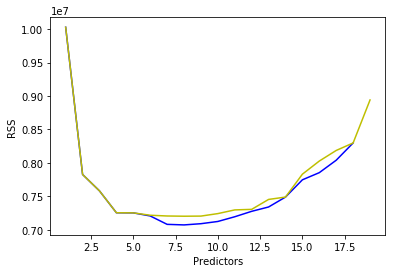
\includegraphics[scale=0.4]{subsetSelection/modelQualification/fig/validatedBestSubsetAndForwardStepwise.png}
	\caption{Best Subset and Forward Stepwise Selection validation set. Best Subset is blue, Forward Stepwise is yellow.}
	\label{fig:validatedBestSubsetAndForwardStepwise}
\end{figure}

\begin{figure}[h]
	\centering
	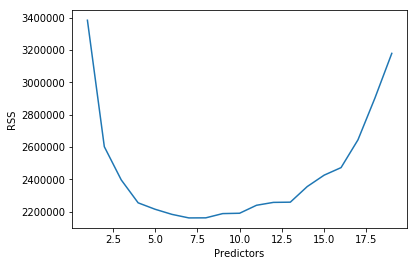
\includegraphics[scale=0.4]{subsetSelection/modelQualification/fig/crossValidation.png}
	\caption{Cross-Validation method with $k=10$.}
	\label{fig:crossValidationRSS}
\end{figure}
